\documentclass[12pt]{article}
\usepackage[top=1in,bottom=1in,left=1in,right=1in]{geometry}
\usepackage{alltt}
\usepackage{array}	
\usepackage{graphicx}
\usepackage{tabularx}
\usepackage{verbatim}
\usepackage{setspace}
\usepackage{listings}
\usepackage{amssymb,amsmath, amsthm}
\usepackage{qtree}
\usepackage{hyperref}
\usepackage{oz}
\usepackage[cc]{titlepic}
\usepackage{fancyvrb}
\usepackage{epstopdf}
\usepackage{soul}
\usepackage{array}
\usepackage{tikz}
\newcolumntype{L}{>{\centering\arraybackslash}m{3cm}}

\title{Concordia University\\
Department of Computer Science and Software Engineering\\
\textbf{SOEN 331 - S and U\\Introduction to Formal Methods\\for Software Engineering}\\
\ \\
\textbf{Assignment 1 - Solutions}\\
Propositional and Predicate Logic, Structures,\\Binary Relations, Functions and Relational Calculus\\
\textbf{Team 19}}
\author{
	\textbf{Samuel Boaknin}\\
	\texttt{40009692}
	\and
	\textbf{Ryan Leyland}\\
	\texttt{40015165}
	\and
	\textbf{Saleha Tariq}\\
	\texttt{40006997}
	\and
	\textbf{Meng Susana Ung}\\
	\texttt{40099729}
}
\date{Date: February 11, 2021}

\begin{spacing}{1.5}
\begin{document}
\maketitle

\newpage
\tableofcontents
\newpage

\section{Solutions}

\subsection{Problem 1 (8 pts)}

\noindent You are shown a set of four cards placed on a table, each of which has a \textbf{number} on one side and a \textbf{symbol} on the other side. The visible faces of the cards show the numbers \textbf{2} and \textbf{7}, and the symbols \textbf{$\Box$}, and \textbf{$\bigcirc$}.

\bigskip
\noindent Which card(s) must you turn over in order to test the truth of the proposition that \textit{``If a card has an odd number on one side, then it has the symbol $\Box$ on the other side''}? Explain your reasoning by deciding for \underline{each} card whether it should be turned over and why.

\bigskip

\noindent \textbf{Solution:}

\noindent Cards to turn over: 7 and \textbf{$\bigcirc$}

\noindent Let p denote odd number on this side of card and q denote \textbf{$\Box$} on opposite side of card then:

7: check this card due to modus ponens

\indent \indent $p \rightarrow q, p \therefore q$

\textbf{$\bigcirc$}: check this card due to modus tollens

\indent \indent $p \rightarrow q, \neg q \therefore \neg p$

2: do not check this card due to inverse error

\indent \indent $p \rightarrow q, \neg p \therefore \neg q$ is incorrect

\textbf{$\Box$}: do not check this card due to converse error

\indent \indent $p \rightarrow q, q \therefore p$ is also incorrect


\newpage

\subsection{Problem 2 (8 pts)}

Consider the predicate \textit{asks(a, b)} that is interpreted as \textit{``a has asked b out on a date.''}
\begin{enumerate}
\item Translate the following into English: $\forall a \exists b~asks(a, b)$ and $\exists b \forall a ~asks(a, b)$.
\item Can we claim that $\forall a \exists b~asks(a, b) \rightarrow \exists b \forall a ~asks(a, b)$? Discuss in detail.
\item Can we claim that $\exists b \forall a ~asks(a, b) \rightarrow \forall a \exists b~asks(a, b)$? Discuss in detail.
\end{enumerate}

\bigskip
\noindent \textbf{Solution:}
\begin{enumerate}
\item \begin{enumerate}
\item $\forall a \exists b~asks(a, b)$ = Everyone has asked at least one person out on a date.
\item $\exists b \forall a ~asks(a, b)$ = There exists a person whom has been asked on a date by everyone.
\end{enumerate}
\item Can we claim that $\forall a \exists b~asks(a, b) \rightarrow \exists b \forall a ~asks(a, b)$? Discuss in detail.

No, modus ponens and modus tollens both fail. There could exist a person whom has not asked the same person out on a date as everyone else. Therefore the LHS
would be true and the RHS false which cannot hold for implication.

\item Can we claim that $\exists b \forall a ~asks(a, b) \rightarrow \forall a \exists b~asks(a, b)$? Discuss in detail.

Yes, if a person has been asked on a date by every person then this implies that every person has asked out at least one person on a date.
\end{enumerate}




\newpage

\subsection{Problem 3 (12 pts)}

\noindent Let $scientist(x)$ denote the statement ``x is a scientist'', and $honest(x)$ denote the statement ``x is honest.'' Formalize the following sentences and indicate their corresponding formal type.

\begin{enumerate}
\item ``No scientists are honest.''

\item ``All scientists are crooked.''

\item ``All scientists are honest.''

\item ``Some scientists are crooked.''

\item ``Some scientists are honest.''

\item ``No scientist is crooked.''

\item ``Some scientists are not crooked.''

\item ``Some scientists are not honest.''

\end{enumerate}

\noindent Identify pairs that are contradictories, contraries, subcontraries, and pairs that support subalteration (clearly indicating superaltern and subaltern).

\bigskip
\noindent \textbf{Solution:}

\noindent The formalization is as follows:

\begin{enumerate}
\item $\forall x (~scientist(x) \implies \neg~honest(x))$ (Type E)
\item $\forall x (~scientist(x) \implies \neg~honest(x))$ (Type E)
\item $\forall x (~scientist(x) \implies ~honest(x))$ (Type A)
\item $\exists x (~scientist(x) \wedge \neg~honest(x))$ (Type O)
\item $\exists x (~scientist(x) \wedge ~honest(x)) (Type I)$
\item $\forall x (~scientist(x) \implies ~honest(x))$ (Type A)
\item $\exists x (~scientist(x) \wedge ~honest(x))$ (Type I)
\item $\exists x (~scientist(x) \wedge \neg~honest(x))$ (Type O)
\end{enumerate}

Statements 1 \& 2 are contradictory with Statements 5 \& 7. Statements 3 \& 6 are contradictory with Statements 4 \& 8. 

Statements 1 \& 2 are contrary with Statements 3 \& 6. Statements 4 \& 8 are subcontrary with Statements 5 \& 7.

Statements 1 \& 2 are superalterns to the subaltern Statements 4 \& 8. Statements 3 \& 6 are superalterns to the subaltern Statements 5 \& 7.



\newpage

\subsection{Problem 4 (12 pts)}

Consider list $\Lambda = \langle w, x, y, z \rangle$, deployed to implement a Queue Abstract Data Type.

\begin{enumerate}

\item Let the head of $\Lambda$ correspond to the front position of the Queue. Implement operations \texttt{enqueue(el, $\Lambda$)} and \texttt{dequeue($\Lambda$)} using list construction operations. In both cases we can refer to $\Lambda'$ as the state of the list upon successful termination of one of its operations.

\item Let us now reverse the way we manipulate our data structure and let the head of $\Lambda$ correspond to the rear of the Queue.
\begin{enumerate}
\item What would be the result of $cons(el, \Lambda)$, and would it be a correct implementation for operation \texttt{enqueue(el, $\Lambda$)}?
\item What would be the result of $list(el, \Lambda)$, and would it be a correct implementation for operation \texttt{enqueue(el, $\Lambda$)}?
\item What would be the result of $concat(list(el), \Lambda)$, and would it be a correct implementation for operation \texttt{enqueue(el, $\Lambda$)}?
\end{enumerate}
\end{enumerate}

\bigskip
\noindent \textbf{Solution:}
\begin{enumerate}
\item \begin{enumerate}
\item \texttt{enqueue(el, $\Lambda$)} : \\\hphantom{Spacer} element = list(el); \\ \hphantom{Spacer} $\Lambda'$ = concat($\Lambda$, element);
\item \texttt{dequeue($\Lambda$)} : \\\hphantom{Spacer} element = head($\Lambda$); \\\hphantom{Spacer} $\Lambda'$ = tail($\Lambda$);
\end{enumerate}
\item \begin{enumerate}
\item $\Lambda' = \langle el, w, x, y, z \rangle$ , Yes correct as new element added to tail of queue
\item $\Lambda' = \langle el, \langle w, x, y, z \rangle \rangle$ , No 'list' function takes elements as parameters, so now there are only two direct elements inside $\Lambda'$
\item $\Lambda' = \langle el, w, x, y, z \rangle$ , Yes correct order, new element added to tail of queue
\end{enumerate}
\end{enumerate}


\newpage

\subsection{Problem 5 (12 pts)}

\noindent Let $A = \{ 0, 1, 2, 3, 4 \}$ and relations $R$, $S$, $T$, and $U$ on $A$ defined as follows:

\[ R = \{ (0, 0),  (0, 1),  (0, 3),  (1, 0),  (1, 1),  (2, 2),  (3, 0),  (3, 1), (3, 3), (4, 0), (4, 1), (4, 3), (4, 4)  \}\]

\[ S = \{ (0, 1),  (1, 1),  (2, 3),  (2, 4), (3, 0), (3, 4), (4, 0), (4, 1), (4, 4)  \}\]

\[ T = \{ (0, 3), (0, 4),  (2, 1), (3, 2), (4, 2), (4, 3) \}\]

\[ U = \{ (0, 0),  (0, 1), (0, 3), (1, 0), (1, 1), (1, 3), (2, 2), (3, 0), (3, 1), (3, 3), (4, 4) \}\]

\noindent Fill in the table below, using $\checkmark$, or $\times$.

\begin{center}
\begin{tabular}{|l|l|l|l|l|l|}
\hline
						&	&	$R$	&	$S$	&	$T$	& $U$\\
\hline
\textbf{Reflexive} 	&	&	$\checkmark$ &	$\times$		&	$\times$ & $\checkmark$\\
\hline
\textbf{Irreflexive} 	&	&	$\times$ &	$\times$		&	$\checkmark$ &	$\times$	\\
\hline
\textbf{Symmetric} 	&	&	$\times$ &	$\times$ 	&	$\times$ &	$\checkmark$\\
\hline
\textbf{Asymmetric} 	&	&	$\times$ &	$\times$ 	&	$\checkmark$ &	$\times$\\
\hline
\textbf{Antisymmetric} &	&	$\times$ &	$\checkmark$	&	$\checkmark$ &	$\times$ \\
\hline
\textbf{Transitive} 	&	&	$\times$ &	$\times$ &	$\times$	&	$\checkmark$\\
\hline
\textbf{Equivalence} 	&	&	$\times$ &	$\times$ &	$\times$	&	$\checkmark$\\
\hline
\textbf{Partial order} 	&	&	$\times$ &	$\times$	&	$\times$	&	$\times$\\
\hline
\end{tabular}
\end{center}

\newpage

\subsection{Problem 6 (8 pts)}

\noindent Consider the relation \textit{``is a subtype of''} over the set \\
\indent \indent \indent $\{ rectangle, quadrilateral, square, parellelogram, rhombus\}$.

\begin{enumerate}

\item Is this an \textit{equivalence relation}?

\item Is this relation a \textit{partial order}? If so, create a \textit{Hasse diagram}, and identify \textit{minimal} and \textit{maximal} elements.

\end{enumerate}

\bigskip
\noindent \textbf{Solution:}

\begin{enumerate}

\item No not an equivalence relation. An equivalence relation must be reflexive, symmetric and transitive. The relation is not symmetric, for example a square is a subtype of a quadrilateral
but a quadrilateral is not a subtype of a square as a square is defined to have four right angled corners.

\item Yes, maximal = quadrilateral \& minimal = square
\end{enumerate}
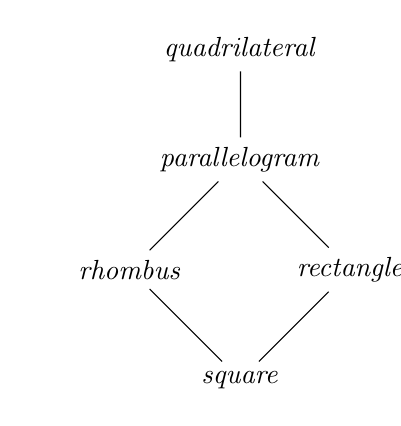
\begin{tikzpicture}[scale=.7]
\indent	\node (one) at (0,4) {$quadrilateral$};
\node (two) at (0,2) {$parallelogram$};
\node (three) at (-2,0) {$rhombus$};
\node (four) at (2,0) {$rectangle$};
\node (five) at (0,-2) {$square$};
\draw (one) -- (two) -- (three) -- (five) -- (four) -- (two);
\end{tikzpicture}


\newpage

\subsection{Problem 7 (8 pts)}

Consider the set $A = \{ w, x, y, z \}$, and the relations

\begin{description}

\item $S = \{ (w, x), (w, y), (x, w), (x, x), (z, x) \}$

\item $T = \{ (w, w), (w, y), (x, w), (x, x),  (x, z), (y, w), (y, y), (y, z) \}$
\end{description}

\noindent Find the following compositions:

\begin{enumerate}
\item $S \circ T$\\
$S \circ T = \{ (w, w), (w, x), (w, y), (w, z), (x, w), (x, x), (x, y), (x, z), (z, w), (z, x), (z, z) \}$\\

\item $T \circ S$\\
$T \circ S = \{ (w, x), (w, y), (x, w), (x, x), (x, y), (y, x) , (y, y) \}$\\

\item $T^{-1} \circ S^{-1}$\\
$T^{-1} \circ S^{-1} = \{ (w, w), (w, x), (w, z), (x, w), (x, x), (x, z), (y, w), (y, x), (z, w), (z, x), (z, z) \}$\\
\end{enumerate}

\noindent \textbf{NOTE}: Some authors (e.g. Rosen) adopt a different ordering of operands than the one we use in our lecture notes. Please follow the ordering (and the definition) of the lecture notes.

\newpage


\subsection{Problem 8 (12 pts)}

Consider sets $A = \{1, 2, 3, 4, 5, 6 \}$ and $B = \{ a, b, c, d, e, f \}$.

\begin{enumerate}

\item Determine the type of the correspondence in each of the following cases, or indicate if the correspondence is not a function.

\begin{enumerate}
\item $\{ 1 \mapsto b, 2 \mapsto c, 3 \mapsto e, 4 \mapsto d, 5 \mapsto f, 3 \mapsto a \}$

\item $\{ 1 \mapsto a, 2 \mapsto d, 3 \mapsto a, 4 \mapsto f, 5 \mapsto d, 6 \mapsto c \}$

\item $\{ 1 \mapsto c, 2 \mapsto b, 3 \mapsto d, 4 \mapsto e, 5 \mapsto e, 6 \mapsto f  \}$

\item $\{ 1 \mapsto b, 2 \mapsto c, 3 \mapsto e, 4 \mapsto d, 5 \mapsto f, 6 \mapsto a \}$
\end{enumerate}

\noindent Fill in the table below, using $\checkmark$, or $\times$.

\begin{center}
\begin{tabular}{|l|c|c|c|c|c|}
\hline
		& Injective		& Surjective	& Bijective 	& \multicolumn{1}{m{3cm}|}{Neither injective nor surjective}	&	Not a function	\\
\hline
(a)		&	$\times$	&	$\times$	&	$\times$	 &	$\times$	&	$\checkmark$  \\
\hline

(b)		&	$\times$	&	$\times$	&	$\times$	&	$\checkmark$	&	$\times$	 \\
\hline


(c)		&	$\times$	&	$\times$	&	$\times$	&	$\checkmark$	&	$\times$  \\
\hline

(d)		&	$\checkmark$	&	$\checkmark$	&	$\checkmark$	&	$\times$	&	$\times$  \\
\hline
\end{tabular}
\end{center}


\item Is it possible to construct a function $f : A \rightarrow B$ which is surjective and not injective?  Discuss.
\end{enumerate}

\noindent No, it is not possible since there are 6 elements in the domain and 6 elements in the codomain. In order for the function to be surjective, each element of the codomain has to be mapped to by at least one element of the domain. If the function were to not be injective, then distinct elements of the domain would be mapped to the same element of the codomain which means that some element or elements of the codomain would not be mapped to by at least one element of the domain since there are equal amounts of elements in the domain and codomain, thus it isn't possible for the surjective function to not be injective.

\newpage

\subsection{Problem 9 (20 pts)}

\noindent Consider the following relation:

\[ laptops : Model \leftrightarrow Brand \]

\noindent where

\[
laptops = \\
\hspace{5mm} \{ \\
\hspace{10mm} legion5 \mapsto lenovo,\\
\hspace{10mm} macbookair \mapsto apple,\\
\hspace{10mm} xps15 \mapsto dell,\\
\hspace{10mm} spectre \mapsto hp,\\
\hspace{10mm} xps13 \mapsto dell,\\
\hspace{10mm} swift3 \mapsto acer,\\
\hspace{10mm} macbookpro \mapsto apple,\\
\hspace{10mm} dragonfly \mapsto hp,\\
\hspace{10mm} envyx360 \mapsto hp\\
\hspace{5mm} \}
\]

\begin{enumerate}

\item What is the domain and the range of the relation?\\
dom $laptops = \{legion5, macbookair, xps15, spectre, xps13, swift3, macbookpro,\\
\hspace*{38mm}dragonfly, envyx360\}$\\\\
ran $laptops = \{ lenovo, apple, dell, hp, acer\}$

\item What is the result of the expression

\[ \{ xps15, xps13, swift3, envyx360 \}  \lhd laptops \]
\[ \{ xps15, xps13, swift3, envyx360 \}  \lhd laptops =\\
\hspace{5mm} \{ \\
\hspace{10mm} xps15 \mapsto dell,\\
\hspace{10mm} xps13 \mapsto dell,\\
\hspace{10mm} swift3 \mapsto acer,\\
\hspace{10mm} envyx360 \mapsto hp\\
\hspace{5mm} \}
\]

\noindent What is the meaning of operator $\lhd$ and where would you deploy such operator in the context of a database management system?\\\\
The $\lhd$ operator restricts the domain of the relation and returns the pairs from the relation where the first element matches one of the elements in the domain restrictor. In the context of a database management system, this domain restriction operator could be used to query the database to determine which \textit{Brands} correspond to certain \textit{Models}, given a specific set of \textit{Models}.

\item What is the result of the expression

\[ laptops \rhd \{ lenovo, hp \} \]
\[ laptops \rhd \{ lenovo, hp \} =\\
\hspace{5mm} \{ \\
\hspace{10mm} legion5 \mapsto lenovo,\\
\hspace{10mm} spectre \mapsto hp,\\
\hspace{10mm} dragonfly \mapsto hp,\\
\hspace{10mm} envyx360 \mapsto hp\\
\hspace{5mm} \}
\]

\noindent What is the meaning of operator $\rhd$ and where would you deploy such operator in the context of a database management system?\\\\
The $\rhd$ operator restricts the range of the relation and returns the pairs from the relation where the second element (\textit{Brand}) matches one of the elements in the range restrictor. In the context of a database management system, this range restriction operator could be used to query the database to determine which \textit{Models} correspond to certain \textit{Brands}, given a specific set of \textit{Brands}.

\item What is the result of the expression

\[ \{ legion5, xps15, xps13, dragonfly \} \ndres laptops \]
\[ \{ legion5, xps15, xps13, dragonfly \} \ndres laptops =\\
\hspace{5mm} \{ \\
\hspace{10mm} macbookair \mapsto apple,\\
\hspace{10mm} spectre \mapsto hp,\\
\hspace{10mm} swift3 \mapsto acer,\\
\hspace{10mm} macbookpro \mapsto apple,\\
\hspace{10mm} envyx360 \mapsto hp\\
\hspace{5mm} \}
\]

\noindent What is the meaning of operator $\ndres$ and where would you deploy such operator in the context of a database management system?\\\\
The $\ndres$ operator performs a domain subtration and removes all pairs from the domain of the relation based on their first elements. In the context of a database management system, this operator could be used to remove pairs from the database based on the name of the first element. Here, we removed \textit{laptops} from the domain of the relation whose \textit{Model} matched the ones with the operator.

\item What is the result of the expression

\[ laptops \nrres \{ apple, dell, hp \} \]
\[ laptops \nrres \{ apple, dell, hp \} =\\
\hspace{5mm} \{ \\
\hspace{10mm} legion5 \mapsto lenovo,\\
\hspace{10mm} swift3 \mapsto acer,\\
\hspace{5mm} \}
\]

\noindent What is the meaning of operator $\nrres$ and where would you deploy such operator in the context of a database management system?\\\\
The $\nrres$ operator performs a range subtration and removes all pairs from the codomain of the relation based on their second elements. In the context of a database management system, this operator could be used to remove pairs from the database based on the name of the second element. Here, we removed \textit{laptops} from the codomain of the relation whose \textit{Brand} matched the ones with the operator.

\item Consider the following expression

\[ laptops \oplus \{ ideapad \mapsto lenovo \} \]

\begin{enumerate}
\item What is the result of the expression?

\[ laptops \oplus \{ ideapad \mapsto lenovo \} =\\
\hspace{5mm} \{ \\
\hspace{10mm} legion5 \mapsto lenovo,\\
\hspace{10mm} macbookair \mapsto apple,\\
\hspace{10mm} xps15 \mapsto dell,\\
\hspace{10mm} spectre \mapsto hp,\\
\hspace{10mm} xps13 \mapsto dell,\\
\hspace{10mm} swift3 \mapsto acer,\\
\hspace{10mm} macbookpro \mapsto apple,\\
\hspace{10mm} dragonfly \mapsto hp,\\
\hspace{10mm} envyx360 \mapsto hp\\
\hspace{10mm} ideapad \mapsto lenovo\\
\hspace{5mm} \}
\]
The relation will have $ideapad \mapsto lenovo$ appended to it.\\

\item What is the meaning of operator $\oplus$ and where would you deploy such operator in the context of a database management system?\\\\
The $\oplus$ operator performs a relational override that adds all elements from the RHS of the operator to the relation, if they do not already exist in the relation. In the context of a database management system, this could be used to update the database and add new elements.\\

\item Does the result of the expression have a permanent effect on the database (relation)? If not, describe in detail how would you ensure a permanent effect.\\\\
This result would not have a permanent effect on the relation, it will only return what the relation would look like with the elements added to it. For a permanent effect, you would need to do
\[ laptops' = laptops \oplus \{ ideapad \mapsto lenovo \} \]

\end{enumerate}

\end{enumerate}


\end{spacing}

\center
\textbf{END OF ASSIGNMENT SOLUTIONS}.



\end{document}
